\documentclass[12pt,t]{beamer}
\usepackage{graphicx}
\setbeameroption{hide notes}
\setbeamertemplate{note page}[plain]
\usepackage{listings}

% set up listing environment
\lstset{language=bash,
        basicstyle=\ttfamily\scriptsize,
        frame=single,
        commentstyle=,
        backgroundcolor=\color{darkgray},
        showspaces=false,
        showstringspaces=false
        }

% get rid of junk
\usetheme{default}
\beamertemplatenavigationsymbolsempty
\hypersetup{pdfpagemode=UseNone} % don't show bookmarks on initial view


% font
\usepackage{fontspec}
\setsansfont
  [ ExternalLocation = ../fonts/ ,
    UprightFont = *-regular , 
    BoldFont = *-bold ,
    ItalicFont = *-italic ,
    BoldItalicFont = *-bolditalic ]{texgyreheros}
\setbeamerfont{note page}{family*=pplx,size=\footnotesize} % Palatino for notes
% "TeX Gyre Heros can be used as a replacement for Helvetica"
% I've placed them in ../fonts/; alternatively you can install them
% permanently on your system as follows:
%     Download http://www.gust.org.pl/projects/e-foundry/tex-gyre/heros/qhv2.004otf.zip
%     In Unix, unzip it into ~/.fonts
%     In Mac, unzip it, double-click the .otf files, and install using "FontBook"

% named colors
\definecolor{offwhite}{RGB}{249,242,215}
\definecolor{foreground}{RGB}{255,255,255}
\definecolor{background}{RGB}{24,24,24}
\definecolor{title}{RGB}{107,174,214}
\definecolor{gray}{RGB}{155,155,155}
\definecolor{subtitle}{RGB}{102,255,204}
\definecolor{hilit}{RGB}{102,255,204}
\definecolor{vhilit}{RGB}{255,111,207}
\definecolor{nhilit}{RGB}{128,0,128}  % hilit color in notes
\definecolor{nvhilit}{RGB}{255,0,128} % vhilit for notes
\definecolor{lolit}{RGB}{155,155,155}

\newcommand{\hilit}{\color{hilit}}
\newcommand{\vhilit}{\color{vhilit}}
\newcommand{\nhilit}{\color{nhilit}}
\newcommand{\nvhilit}{\color{nvhilit}}
\newcommand{\lolit}{\color{lolit}}

% use those colors
\setbeamercolor{titlelike}{fg=title}
\setbeamercolor{subtitle}{fg=subtitle}
\setbeamercolor{institute}{fg=gray}
\setbeamercolor{normal text}{fg=foreground,bg=background}
\setbeamercolor{item}{fg=foreground} % color of bullets
\setbeamercolor{subitem}{fg=gray}
\setbeamercolor{itemize/enumerate subbody}{fg=gray}
\setbeamertemplate{itemize subitem}{{\textendash}}
\setbeamerfont{itemize/enumerate subbody}{size=\footnotesize}
\setbeamerfont{itemize/enumerate subitem}{size=\footnotesize}

% page number
\setbeamertemplate{footline}{%
    \raisebox{5pt}{\makebox[\paperwidth]{\hfill\makebox[20pt]{\lolit
          \scriptsize\insertframenumber}}}\hspace*{5pt}}

% add a bit of space at the top of the notes page
\addtobeamertemplate{note page}{\setlength{\parskip}{12pt}}

% default link color
\hypersetup{colorlinks, urlcolor={hilit}}

% a few macros
\newcommand{\bi}{\begin{itemize}}
\newcommand{\bbi}{\vspace{24pt} \begin{itemize} \itemsep8pt}
\newcommand{\ei}{\end{itemize}}
\newcommand{\ig}{\includegraphics}
\newcommand{\subt}[1]{{\footnotesize \color{subtitle} {#1}}}
\newcommand{\ttsm}{\tt \small}
\newcommand{\ttfn}{\tt \footnotesize}
\newcommand{\figh}[2]{\centerline{\includegraphics[height=#2\textheight]{#1}}}
\newcommand{\figw}[2]{\centerline{\includegraphics[width=#2\textwidth]{#1}}}


%%%%%%%%%%%%%%%%%%%%%%%%%%%%%%%%%%%%%%%%%%%%%%%%%%%%%%%%%%%%%%%%%%%%%%
% end of header
%%%%%%%%%%%%%%%%%%%%%%%%%%%%%%%%%%%%%%%%%%%%%%%%%%%%%%%%%%%%%%%%%%%%%%

% title info
\title{Unix command line; editors}
\subtitle{Tools for Reproducible Research}
\author{\href{http://www.biostat.wisc.edu/~kbroman}{Karl Broman}}
\institute{Biostatistics \& Medical Informatics, UW{\textendash}Madison}
\date{\href{http://www.biostat.wisc.edu/~kbroman}{\tt \scriptsize \color{foreground} biostat.wisc.edu/{\textasciitilde}kbroman}
\\[-4pt]
\href{http://github.com/kbroman}{\tt \scriptsize \color{foreground} github.com/kbroman}
\\[-4pt]
\href{https://twitter.com/kwbroman}{\tt \scriptsize \color{foreground} @kwbroman}
\\[-4pt]
{\scriptsize Course web: \href{http://bit.ly/tools4rr}{\tt bit.ly/tools4rr}}
}


\begin{document}

% title slide
{
\setbeamertemplate{footline}{} % no page number here
\frame{
  \titlepage

\note{My goal in this lecture is to convince you that  \\
(a) command-line-based tools are the things to focus on, \\
(b) you need to choose a powerful, universal text editor (you'll use
  it a lot), \\
(c) you want to be comfortable and skilled with each.

For your work to be reproducible, it needs to be code-based;
don't touch that mouse!
}
} }


\begin{frame}[c]{}


\centering
\Large

Windows {\color{lolit} vs.} Mac OSX {\color{lolit} vs.} Linux

\bigskip
\bigskip

Remote {\color{lolit} vs.} Not

\note{The Windows operating system is not very programmer-friendly.

Mac OSX isn't either, but under the hood, it's just unix.

Don't touch the mouse! Open a terminal window and start typing.

I do most of my work directly on my desktop or laptop. You might
prefer to work remotely on a server, instead. But I can't stand having
any lag in looking at graphics.
}
\end{frame}


\begin{frame}[c]{If you're stuck with Windows...}

\centering
\Large

Consider \href{http://www.cygwin.org}{Cygwin}
{\color{lolit} (and perhaps \href{https://code.google.com/p/mintty/}{Mintty})}

\note{Cygwin is an effort to get Unix command-line tools in Windows.

Mintty is a terminal emulator.}
\end{frame}

\begin{frame}[c]{If you use a Mac...}

\centering
\Large

Consider \href{http://brew.sh/}{Homebrew} and
\href{http://www.iterm2.com}{iTerm2}

\note{Homebrew is a packaging system; iTerm2 is a Terminal replacement.

I do all of my work on a Mac (except really big computational jobs),
and there are a lot of different tools that I like and would recommend:

divvy, http://mizage.com/divvy \\
caffeine, http://lightheadsw.com/caffeine \\
bartender, http://www.macbartender.com \\
hazel, http://www.noodlesoft.com/hazel.php \\
launchbar, http://www.obdev.at/products/launchbar/index.html \\
simplenote, http://simplenote.com \\
jumpcut, http://jumpcut.sourceforge.net \\
color oracle, http://colororacle.org \\
textexpander, http://smilesoftware.com/TextExpander
}

\end{frame}


\begin{frame}{The command line is your friend}

\vspace{24pt}

\bi
\itemsep24pt
\item Don't touch that mouse!
\item Scriptable
\item Flexible
\ei
\note{In the long run, you'll be happier, having conquered the command line.

Pointing-and-clicking is not reproducible, and every time you take
your hands off the keyboard, there's a loss of efficiency.

The command line allows you to piece together multiple tools and so do
things that weren't anticipated by the developer of the GUI.

And it's only through scripts that you'll have truly reproducible
analyses.
}
\end{frame}



\begin{frame}[c]{The shell}


\centerline{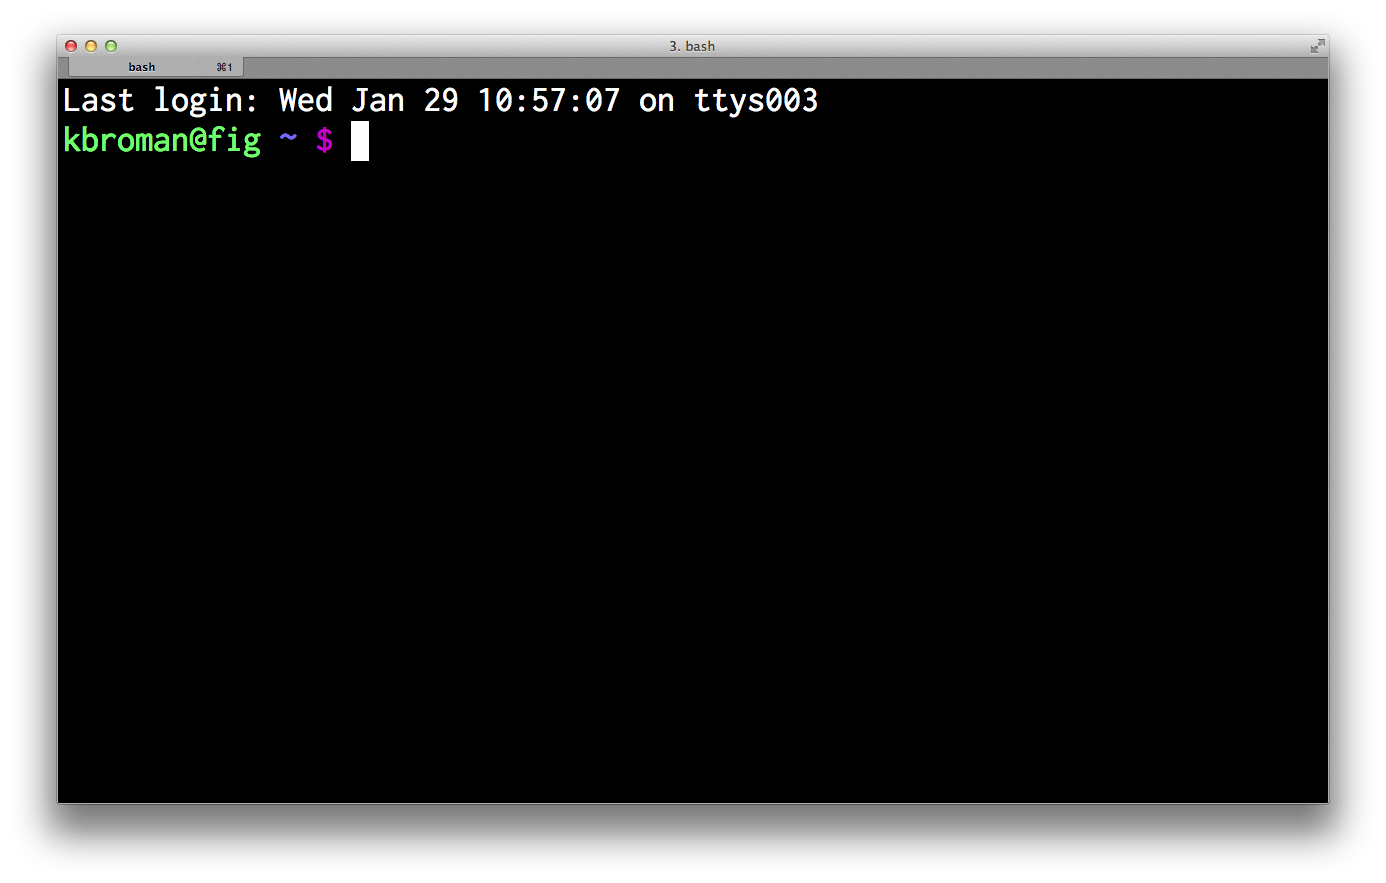
\includegraphics[width=\textwidth]{Figs/shell.png}}

Options: \href{http://en.wikipedia.org/wiki/Tcsh}{tcsh}, \href{http://www.gnu.org/software/bash/manual/bashref.html}{bash}, \href{http://www.zsh.org/}{zsh}


\note{The shell is a program -- an interface to the operating
  system.

There are a number to choose from. I use {\tt bash}; I've heard great
things about {\tt zsh}.
}

\end{frame}



\begin{frame}{Basics}

\vspace{18pt}
\bi
\itemsep18pt
\item Directory structure

{\color{lolit} Absolute vs. relative paths

\tt ls -l {\textasciitilde}/.. }

\item Creating, removing, changing directories

{\tt \color{lolit} mkdir

rmdir

cd

cd -}

\item Moving, copying, removing files

{\tt \color{lolit} mv

cp

rm -i}

\ei

\note{This stuff is too boring to spend much time on.

But I should emphasize the importance of using relative paths (e.g.,
{\tt ../Figs/fig1.pdf}) in a project; reliance on absolute paths
(e.g., {\tt {\textasciitilde}/Projects/Blah/Figs/fig1.pdf}) make life difficult when
you move the project to a different system.
}

\end{frame}


\begin{frame}[fragile]{{\tt {\textasciitilde}/.bash\_profile}}

\vspace{-12pt}

\begin{semiverbatim}
\begin{lstlisting}
export PATH=.:/usr/local/bin:$PATH
export LD_LIBRARY_PATH=/usr/local/lib

noclobber=1    # prevent overwriting of files
IGNOREEOF=1    # disable Ctrl-D as a way to exit
HISTCONTROL=ignoredups

alias cl='clear;cd'
alias rm='rm -i'
alias mv='mv -i'
alias cp='cp -i'
alias ls='ls -GF'
alias 'l.'='ls -d .[a-zA-Z]*'
alias ll='ls -lh'
alias md='mkdir'
alias rd='rmdir'
alias rmb='rm .*~ *~ *.bak *.bk!'

alias Rb='R CMD build --force --resave-data'
alias Ri='R CMD INSTALL --library=/Users/kbroman/Rlibs'
alias Rc='R CMD check --library=/Users/kbroman/Rlibs'
alias Rcc='R CMD check --as-cran --library=/Users/kbroman/Rlibs'
\end{lstlisting}
\end{semiverbatim}


\note{Use the {\tt .bash\_profile} file to define various
  variables and aliases to make your life easier.

The most important variable is {\tt PATH}: it defines the set of
directories where the shell will look for executable programs.

If ``{\tt .}'' isn't part of your {\tt PATH}, you'll need to type
something like {\tt ./myscript.py} to execute a script in your working
directory. So put ``{\tt .}'' in your {\tt PATH}.

My {\tt .bash\_profile} file sources a {\tt .bashrc} file; I don't
quite understand when one is used versus the other. Google ``{\tt .bashrc
vs .bash\_profile}.''

There are links to my {\tt .bash\_profile} and {\tt .bashrc} files on
the resources page at the course web site; some of it might just be
total crap.

Important note: use of aliases within your code will create
reproducibility issues; another user will need those same aliases.
Consider testing your code on a more basic account.
}

\end{frame}


\begin{frame}[fragile]{Redirection and pipes}

\begin{semiverbatim}
\begin{lstlisting}
$ locate article.cls > output.txt
$ locate book.cls >> output.txt
$ grep texmf output.txt

$ locate article.cls | grep texmf

$ locate article.cls | grep texmf | less

$ locate article.cls | wc -l
$ locate article.cls | grep texmf | wc -l

$ cat file1.txt file2.txt > combined.txt
\end{lstlisting}
\end{semiverbatim}

\note{Use $>$ to redirect output ``stdout'' to a file.

Use $>>$ to redirect output and append to the file.

Use $<$ to have input ``stdin'' come from a file.

Use $|$ to have the output of one command made the input to
another.

A key design principle in Unix is the piecing together of small commands using
this sort of technique. There are lots of little commands (often with
short, cryptic names) that can be combined together with great
flexibility.

Important tools mentioned here: {\tt locate} (find files matching a
pattern), {\tt grep} (search for patterns in a file), {\tt less} (look
through long files a page at a time),
{\tt wc} (count the number of words, lines and/or characters in a
file),
{\tt cat} (print contents of or concatenate text files)
}

\end{frame}




\begin{frame}[fragile]{Wild cards}

\begin{semiverbatim}
\begin{lstlisting}
$ grep blah *.txt

$ ls blah.???

$ ls [a-z]*

$ ls /usr/bin/[auz]*

$ ls /usr/bin/[auz]*.*
\end{lstlisting}
\end{semiverbatim}

\note{{\tt *} stands for anything

{\tt ?} stands for a single character

Use {\tt []} to match some specific set or range of characters}
\end{frame}


\begin{frame}[fragile]{Suspend/foreground/background}

\begin{semiverbatim}
\begin{lstlisting}
$ R CMD BATCH input.R output.txt &

$ R CMD BATCH input.R output.txt
[ctrl-Z]
$ bg

$ emacs afile.txt
[ctrl-Z]
$ fg
\end{lstlisting}
\end{semiverbatim}

\note{Use {\tt \&} to run a job in the background.

Use ctrl-Z to suspend the current job. Then use {\tt bg} to then put it in
the background or {\tt fg} to bring it back to the foreground.

I use ctrl-Z and {\tt bg} if I had forgotten to use {\tt \&}.

I use ctrl-Z with emacs sometimes, to do some command-line things
without opening another shell/terminal; I'll then use {\tt fg} to
bring emacs back. Or I'll forget about it and muck a bunch of stuff
up.
}
\end{frame}


\begin{frame}[fragile]{Other useful tools}

\begin{semiverbatim}
\begin{lstlisting}
$ find . -name *.py

$ ps ux

$ top

$ df -hk

$ du -h
$ du -hd2

$ ln -s ~/Projects/SomeFriend/Data
$ ln -s ~/Projects/SomeFriend/Data SomeFriend_Data

$ tar xzvf qtl_1.29-2.tar.gz
$ tar czvf blah.tgz Blah/
$ tar tzvf blah.tgz

$ wget http://kbroman.github.io/Tools4RR/pages/resources.html
\end{lstlisting}
\end{semiverbatim}

\note{{\tt find} is like {\tt locate}

{\tt ps ux} to see what processes are running.

{\tt top} gives an interactive view of what processes are running.

{\tt df -hk} shows disk usage

{\tt du -hd2} shows disk usage in a directory and its subdirectories;
the {\tt d2} bit says go no more than 2 levels down through the subdirectories.

{\tt ln -s} makes a ``soft link'' to a file or directory. It acts like
there's a copy, but it's not really copied.

{\tt tar} is used to archive a bunch of files within a single
file. {\tt x} for extract, {\tt c} for combine, {\tt t} for test, {\tt
  z} for compress/zip, {\tt v} for verbose, {\tt f} for ``file name to follow.''

{\tt wget} (see also {\tt curl}) for grabbing something from the web.
}

\end{frame}


\begin{frame}[fragile]{Further useful tools}

\vspace{-12pt}

\begin{semiverbatim}
\begin{lstlisting}
$ whereis bash
$ type rm
$ type emacs

$ pwd

$ head afile.txt
$ tail afile.txt
$ head -n20 afile.txt

$ man head

$ kill 8453
$ kill -9 8453

$ history
$ !!
$ !-2
$ !503

$ ping www.google.com

$ ispell afile.txt
\end{lstlisting}
\end{semiverbatim}

\note{{\tt whereis} for finding a program. \\
{\tt type} for figuring out the location of a program or the
definition of an alias.

{\tt pwd} -- print working directory

{\tt head} -- print first few lines of a file \\
{\tt tail} -- print the last few lines of a file

{\tt man} -- view manual page

{\tt kill} -- kill a job

{\tt history} -- view command history \\
{\tt !} -- execute past commands

{\tt ping} -- see if you can connect to some server

{\tt ispell} -- spell checker
}

\end{frame}


\begin{frame}[c]{Moving around the command line}

\renewcommand{\arraystretch}{1.3}
\begin{tabular}{ll}
{\tt ctrl-f, ctrl-b} & \color{lolit} move forward and back \\
{\tt ctrl-a, ctrl-e} & \color{lolit}  move to beginning and end of line \\
{\tt ctrl-k, ctrl-u} & \color{lolit}  delete rest of line, or to the start \\
{\tt ctrl-l} & \color{lolit}  clear the screen \\
{\tt ctrl-c} & \color{lolit}  cancel what you've typed \\
{\tt tab} & \color{lolit}  autocomplete command or file \\
{\tt ctrl-p, ctrl-n} & \color{lolit}  forward and backward in history \\
{\tt ctrl-r} & \color{lolit}  search for a previous command
\end{tabular}

\note{These are mostly emacs-like key ``bindings''.}
\end{frame}



\begin{frame}[c]{File modes}

\centerline{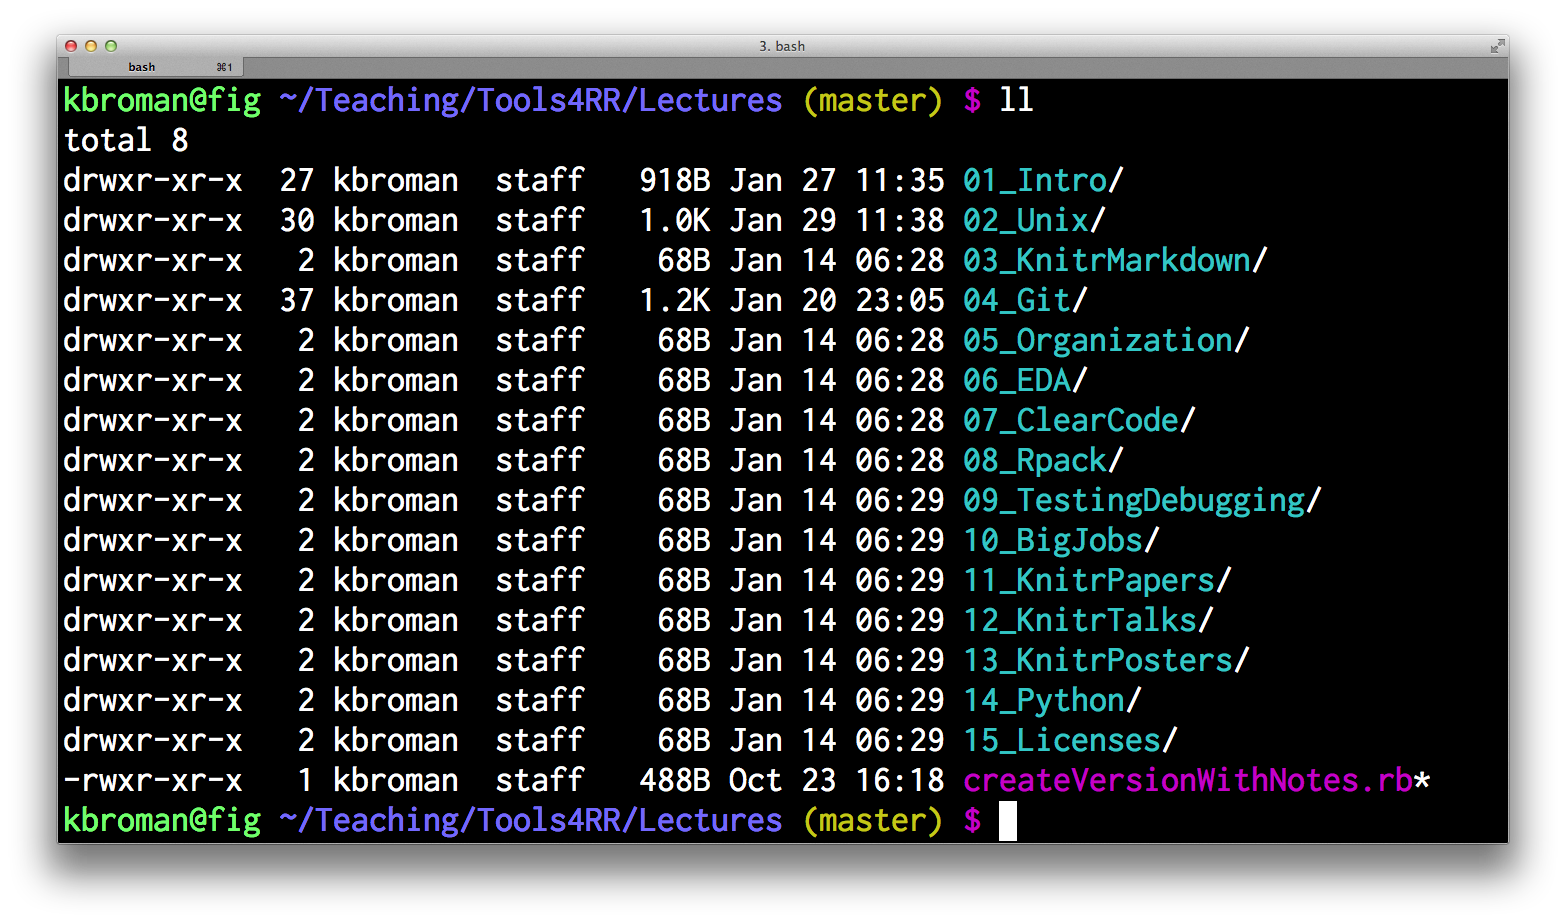
\includegraphics[width=\textwidth]{Figs/chmod.png}}

\note{Note the mode, owner, and group for each file.

mode = read/write/executable for owner/group/everyone

r = readable; w = writable; x = executable (for a directory, enter-able)}
\end{frame}


\begin{frame}{File modes/owner/group}

\vspace{24pt}

\tt sudo chown kbroman .

chgrp -R staff .

chmod +x createVersionWithNotes.rb

chmod 755 02\_Unix

chmod 644 02\_Unix/02\_unix.tex

chmod 700 Private\_stuff

\note{You don't usually need to change the owner or group assigned to
  a file or directory, but it's good to be aware of the
  possibility.

  Groups are useful if you want a file accessible by some set of
  people but not everyone. You need a system admin to set up the group.

  You often want to make scripts executable, or make files/directories
  unreadable or unwriteable.

  For example, primary raw data files should not be writable. Large
  Excel-based data files often contain screwed up cells where someone
  was typing in some random spot without realizing it. I found myself
  doing that yesterday!

  The octal codes (e.g, 755 and 644) are convenient, once
  you get the hang of them.}

\end{frame}


\begin{frame}{How to solve computing problems}

\vspace{24pt}

\bi
\item {\color{vhilit} Try stuff!}
\item man pages and help files
\item {\tt blah -h} or {\tt blah --help}
\item \href{http://www.google.com}{Google}
\item \href{http://stackoverflow.com}{Stackoverflow} and other
  \href{http://stackexchange.com}{StackExchange} sites
\item \href{http://www.google.com}{Google} with {\tt site:stackoverflow.com}
\item email lists and google groups
\item friends or colleagues
\item \href{http://twitter.com}{Twitter}
\item Buy a book. Buy {\color{vhilit} all} of the books.
\ei

\note{You will run into crazy and mysterious errors. Will you give up, or
  figure them out?

  Rule number 1: try stuff. Figure out how something works by trying
  it out in different ways.

  Rule number 2: Google. Google the exact error message, or a part of
  an error message. You'll often get to a stackexchange site; don't
  forget to read the comments as well as the answers. Often the best
  answer is in a comment.

  Rule number 3: Ask for help. Talk to your friends. Talk to me.
  Post a question at a stackexchange site.

  I'm a relatively recent convert to Twitter. I focus on just a few
  things that interest me (mostly academic publishing, reproducible
  research, and interactive graphics). If you tweet a question, you'll
  be surprised at how quickly you get an answer.

  I do tend to buy all possible books on a topic that is of even
  passing interest to me. I read at least part of each of them.
}
\end{frame}


\begin{frame}{Examples}

\vspace{24pt}

\bi
\item How do you suppress warnings in knitr?
\item What symbol corresponds to the unicode {\tt {\textbackslash}u00B1}?
\item What's the difference between {\tt curl} and {\tt wget}?
\item What does "{\tt 502 Bad Gateway}" mean?
\item "{\tt To open gs you need to install X11}"
\item {\tt mclapply} isn't working in Windows
\item How to ping a server in Python?
\item {\tt Font shape `EU1/pplx/m/n' undefined}
\item {\tt except KeyError, k: raise AttributeError, k}
\ei

\note{These are examples of things you might search for.

If you don't understand an error message, start by pasting it into
google.
}
\end{frame}


\begin{frame}[c]{Important principle}

\centerline{Learn to code by looking at good code.}

\note{Identify programmers that you respect (e.g., Hadley Wickham),
  and study what they do.
}
\end{frame}



\begin{frame}{Choose a good editor}

\vspace{24pt}

\bi
\itemsep12pt
\item \href{http://www.emacswiki.org/emacs/}{Emacs}
\item \href{http://www.vim.org/}{VIM}
\item \href{http://www.rstudio.com/ide/}{RStudio}
\item \href{http://www.barebones.com/products/textwrangler/}{Textwrangler}
\item \href{http://notepad-plus-plus.org/}{Notepad++}
\item \href{http://sourceforge.net/projects/tinn-r/}{Tinn-R}
\ei

\note{I use emacs; I should probably use vim.

  RStudio is increasingly
  useful, but as a general editor (for things that aren't R), I think
  it's insufficient.

  The choice of editor is very personal.
}
\end{frame}


\begin{frame}{A good editor}

\vspace{24pt}

\bi
\itemsep12pt
\item Doesn't require pointing-and-clicking
\item Easy to get code between R and a script
\item Syntax highlighting of code
\item Automatic indentation
\item Close parentheses/brackets/braces
\item Browse code across files
\item Integrated with other tools (e.g., version control)
\ei

\note{I've not figured out how to explore code across a set of files
  in emacs; otherwise I'm very happy with it.
}
\end{frame}


\begin{frame}[c]{Don't forget to look at the resources page}


\centerline{\href{http://kbroman.github.io/Tools4RR/pages/resources.html}{\tt http://kbroman.github.io/Tools4RR/pages/resources.html}}

\note{If you find other useful resources, let me know.

When we get to git and GitHub, make a pull request!
}
\end{frame}


\end{document}
